\documentclass{beamer}
\usepackage[utf8]{inputenc}
\usepackage{algorithmic}
\usepackage{algorithm}
\usepackage{booktabs}
\usepackage{textcomp}
\usepackage{amsfonts}
\usepackage{amssymb}
\usepackage{courier}
\usepackage{tikz}
\usepackage{soul}
\usepackage{graphicx}
\usepackage{listings}
\usepackage{makecell}
\usepackage{mathtools}
\usepackage[font={small},
            labelfont={color=black}]{caption}
\usetheme{Rochester}

\usefonttheme[onlymath]{serif}
\beamertemplatenavigationsymbolsempty
\setbeamertemplate{caption}[numbered]
\title{\Large{\textbf{A C\texttt{++} Concepts Primer:}}\\
       \large{\emph{defining and applying constraints}}}
\author{\vspace{2ex}\\
        \textbf{Erik Sven Vasconcelos Jansson}\\
        {\href{mailto:erik.s.v.jansson@tum.de}
        {\texttt{<erik.s.v.jansson@tum.de>}}} \\
        {at Technical University of Munich}}

\lstset{basicstyle=\footnotesize\ttfamily,
        breakatwhitespace = false,
        breaklines = true,
        keepspaces = true,
        language = C++,
        showspaces = false,
        showstringspaces = false,
        frame = tb,
        numbers = left,
        numbersep = 5pt,
        xleftmargin = 16pt,
        framexleftmargin = 16pt,
        escapeinside={<@}{@>},
        morekeywords = {
            concept,
            requires,
            T, U, N,
            point2,
            vector,
            noexcept,
            size_t,
            decltype
        }}

\let\svthefootnote\thefootnote
\textheight 1in
\newcommand\blankfootnote[1]{%
  \let\thefootnote\relax\footnotetext{#1}%
  \let\thefootnote\svthefootnote%
}
\let\svfootnote\footnote
\renewcommand\footnote[2][?]{%
  \if\relax#1\relax%
    \blankfootnote{#2}%
  \else%
    \if?#1\svfootnote{#2}\else\svfootnote[#1]{#2}\fi%
  \fi
}

\usepackage{etoolbox}
\makeatletter
\patchcmd{\endbeamer@frameslide}{\ifx\beamer@frametitle\@empty}{\iffalse}{}{\errmessage{failed to patch}}
\makeatother

\addtobeamertemplate{frametitle}{}{%
\begin{tikzpicture}[remember picture,overlay]
\node[anchor=north east,yshift=-7pt,xshift=-5pt] at (current page.north east) {\includegraphics[height=0.7cm]{figures/tulogo}};
\end{tikzpicture}}

\setbeamerfont{bibliography item}{size=\tiny}
\setbeamerfont{bibliography entry author}{size=\tiny}
\setbeamerfont{bibliography entry title}{size=\tiny}
\setbeamerfont{bibliography entry location}{size=\tiny}
\setbeamerfont{bibliography entry note}{size=\tiny}
\renewcommand*{\thefootnote}{\fnsymbol{footnote}}
\setbeamertemplate{footline}[frame number]

\makeatletter
\let\@@magyar@captionfix\relax
\makeatother

\begin{document}
    \frame{\titlepage}
    \begin{frame}[fragile]{Presentation Outline}
        \begin{columns}
        \column{0.52\textwidth}
            \begin{enumerate}
                \item Generic programming in C\texttt{++} \begin{itemize}
                    \item{\underline{unconstrained} templates.}
                \end{itemize}
                \item Problems and some solutions \begin{itemize}
                    \item{read the documentation,}
                    \item{type traits plus SFINAE,}
                    \item{... arcane ``magic'' code.}
                \end{itemize}
                \item How \textbf{Concepts Lite} improve \begin{itemize}
                    \item{\textcolor{red}{\st{un}}\underline{constrained} templates.}
                \end{itemize}
            \item \emph{Applying concept constraints} \begin{itemize}
                    \item using \texttt{requires} clause,
                    \item overload with constraint,
                    \item operations on constraint.
                \end{itemize}
            \end{enumerate}
        \column{0.48\textwidth}
            \begin{enumerate}
                \setcounter{enumi}{4}
                \item \emph{Defining list of constraints} \begin{itemize}
                    \item \texttt{requires} expressions, \begin{itemize}
                        \item simple,
                        \item type,
                        \item compound,
                        \item nested.
                    \end{itemize}
                    \item requirement\, evaluation,
                    \item naming with \texttt{concept},
                    \item defining good concepts.
                \end{itemize}
                \item Standard Library Concepts
                \item Terse syntaxes for C\texttt{++}20?
                \item Summary, post-Rapperswil
            \end{enumerate}
        \end{columns}
    \end{frame}

    \begin{frame}[fragile]{Generic Programming}
        C\texttt{++} is a rich multi-paradigm language, supporting both \emph{run time} and \emph{compile-time polymorphism}. At compile-time, \emph{templates} give support for \emph{generic programming}. However, templates are fragile, unlike their run time counterpart, because they are \emph{unconstrained}. This leads to \emph{bad error messages}, \emph{unclear interfaces}, and \underline{violence}.

        \vspace{1em}
        Let's build up an example of the current state of generics in C\texttt{++}, and see where they \emph{succeed} \& \emph{fail}; and where \emph{concepts} may help!
    \end{frame}

    \begin{frame}[fragile]{Regular Programming}
        \framesubtitle{Generic Programming}
        Consider this function below, what does it do? How do you know? \textbf{Note:} this is not a very good implementation, e.g. \texttt{p > q} is bad.
        \begin{center}
        \begin{lstlisting}[caption={a ``mysterious'' function; can you figure out what this code is?}]
double f(const double* p,
         const double* const q) {
    double x {  };
    const double s = q - p;
    while (p != q)
        x += *p++;
    return x / s;
} \end{lstlisting}
        \end{center}
    \end{frame}

    \begin{frame}[fragile]{Operator Overloading}
        \framesubtitle{Generic Programming}
        We can make ``similarly behaving things'', have the same syntaxes.
        \begin{center}
        \begin{lstlisting}[caption={boilerplate for the next example; a very incomplete point class.}]
struct point2 {
    double x, y;
    point2& operator+=(const point2& p);
};

point2& point2::operator+=(const point2& p) {
    x += p.x; y += p.y;
    return *this;
}

point2 operator/(const point2& p, double s) {
    return { p.x / s, p.y / s };
} \end{lstlisting}
        \end{center}
    \end{frame}

    \begin{frame}[fragile]{Mysterious Functions?}
        \framesubtitle{Generic Programming}
        Consider this function below, what does it do? How do you know? \textbf{Note:} this is not a very good implementation, e.g. \texttt{p > q} is bad.
        \begin{center}
        \begin{lstlisting}[caption={another mysterious, yet strangely familiar function (déjà vu?).}]
point2 f(const point2* p,
         const point2* const q) {
    point2 x {  };
    const double s = q - p;
    while (p != q)
        x += *p++;
    return x / s;
} \end{lstlisting}
        \end{center}
    \end{frame}

    \begin{frame}[fragile]{Template Parameters}
        \framesubtitle{Generic Programming}
        Obviously, both functions are finding the mean/average somehow. Since both have the same syntax (thanks to operator overloading) we can ``lift'' the implementation. Now, what is \emph{required} from \textbf{\texttt{T}}?
        \begin{center}
            \begin{lstlisting}[caption={natural generalization of the function from the previous slides.}]
template<typename T>
T mean(const T* begin,
       const T* const end) {
    T sum {  };
    const double size = end - begin;
    while (begin != end)
        sum += *begin++;
    return sum / size;
} \end{lstlisting}
        \end{center}
    \end{frame}

    \begin{frame}[fragile]{Comically Bad Errors}
        \framesubtitle{Generic Programming}
        Because \emph{requirements} of unconstrained templates aren't explicit, a user which hasn't understood the interface may get horrible errors because the syntax is checked \textbf{after} \emph{template instantiation}. Which might be deeply nested. Can't we check \textbf{before} instantiating this?
        \begin{center}
            \begin{lstlisting}[caption={classic code examples that give ``bad'' template error messages.}]
std::list l { 5, 1, 4, 3, 2 };
std::sort(l.begin(), l.end());
// <@\texttildelow @>48 lines of errors in gcc.

struct Widget {  };

std::set<Widget> w;
w.insert(Widget{});
// <@\texttildelow @>412 lines here.\end{lstlisting}
        \end{center}
    \end{frame}

    \begin{frame}[fragile]{Parameter Predicates}
        \framesubtitle{Generic Programming}
        Here we have \emph{constrained} the template parameter list, allowing the compilers to check requirements \textbf{before} instantiating the template.
        \begin{center}
        \begin{lstlisting}[caption={constraining the function template using a \texttt{requires} clause.}]
template<typename T> requires DefaultConstructible<T>
                              && SummableWith<T,T> &&
                              ScalableWith<T, double>
T mean(const T* begin,
       const T* const end) {
    T sum {  };
    const double size = end - begin;
    while (begin != end)
        sum += *begin++;
    return sum / size;
} \end{lstlisting}
        \end{center}
    \end{frame}

    \begin{frame}[fragile]{Problems and Solutions}
        Before considering concepts, let's look at how we currently solve the problems we've discussed, and where these fall short. As you will shortly see, specifying constraints by concept is vastly better.
        \vspace{1em}
        \begin{itemize}
            \item{\textbf{Just read the documentation:} good luck with that, even when people read it, they might implement it incorrectly :(}
            \item{\textbf{Type traits and SFINAE:} powerful, and works in many of the cases we use concepts. \textbf{Not} easy to specify constraints.}
            \item{\textbf{Tag dispatching plus libraries:} hacky, not discussed here.}
        \end{itemize}
    \end{frame}

    \begin{frame}[fragile]{Read the Specifications}
        \framesubtitle{Problems and Solutions}
        \begin{center}
        \begin{table}
        \begin{tabular}{ccc}
            \toprule
            \bf{Expression} & \bf{Return Value is} & \bf{Requirements Specification} \\
            \midrule
            \texttt{x == y} & \texttt{bool} convertible & \makecell[l]{\texttt{==}\, is an equivalence relation,\\
                                                                       that is, satisfies the following:\\
                                                                       $\rightarrow$ for all \texttt{x}, \texttt{x == x} is satis.,\\
                                                                       $\rightarrow$ if \texttt{x == y}, then \texttt{y == x},\\
                                                                       $\rightarrow$ if \texttt{x == y}, and\; \texttt{y == z},\\
                                                                       \;\;\;\, then \texttt{x == z}, follows too.
                                                                       } \\
            \bottomrule
        \end{tabular}
        \caption{\texttt{EqualityComparable} requirements from the C\texttt{++} standard.}
        \end{table}
        \end{center}
    \end{frame}

    \begin{frame}[fragile]{Type Trait and SFINAE}
        \framesubtitle{Problems and Solutions}
        \begin{center}
        \begin{lstlisting}[caption={expressing \texttt{EqualityComparable} as a SFINAE type trait.}]
template<typename T, typename U, typename = void>
struct is_equality_comparable : std::false_type {  };

template<typename T, typename U>
struct is_equality_comparable<T, U,
    typename std::enable_if<true,
    decltype(std::declval<T&>() == std::declval<U&>()
             ,(void)0)>::type> : std::true_type {  };\end{lstlisting}
        \end{center}
    \end{frame}

    \begin{frame}[fragile]{Concepts to the Rescue}
        \framesubtitle{Problems and Solutions}
        \begin{center}
        \begin{lstlisting}[caption={\texttt{EqualityComparable} concept which ``satisfies''\footnote{not really; see the Ranges TS, this is \texttt{WeaklyEqualityComparable} \texttt{:)}} Table 1.}]
template<typename T, typename U>
concept EqualityComparable = requires(T x, U y) {
    { x == y } -> bool;
    { x != y } -> bool;
    { y != x } -> bool;
    { y == x } -> bool;
}; \end{lstlisting}
        \end{center}
    \end{frame}

    \begin{frame}[fragile]{Overloading by SFINAE?}
        \framesubtitle{Problems and Solutions}
        \begin{center}
        \begin{lstlisting}[caption={overloading the constructor by using SFINAE \& type traits...}]
struct Factory {
    enum { INTEGRAL, FLOATING } m_type;

    template<typename T,
             typename = std::enable_if<
             std::is_integral_v<T>>
    Factory(T) : m_type { INTEGRAL } {}
    template<typename T,
             typename = std::enable_if<
             std::is_floating_point_v<T>>
    Factory(T) : m_type { FLOATING } {}
}; \end{lstlisting}
        \end{center}
    \end{frame}

    \begin{frame}[fragile]{Overloading by SFINAE}
        \framesubtitle{Problems and Solutions}
        \begin{center}
        \begin{lstlisting}[caption={...doesn't work if we don't use a \texttt{dummy} for disambiguation.}]
struct Factory {
    enum { INTEGRAL, FLOATING } m_type;
    template<int> struct dummy { dummy(int) {  } };
    template<typename T,
             typename = std::enable_if<
             std::is_integral_v<T>>
    Factory(T, dummy<0>=0) : m_type { INTEGRAL } {}
    template<typename T,
             typename = std::enable_if<
             std::is_floating_point_v<T>>
    Factory(T, dummy<1>=0) : m_type { FLOATING } {}
}; \end{lstlisting}
        \end{center}
    \end{frame}

    \begin{frame}[fragile]{Concepts to the Rescue}
        \framesubtitle{Problems and Solutions}
        \begin{center}
        \begin{lstlisting}[caption={overloading based on constraint with the \texttt{requires} clause.}]
struct Factory {
    enum { INTEGRAL, FLOATING } m_type;
    template<typename T> requires Integral<T>
    Factory(T) : m_type { INTEGRAL } {}
    template<typename T> requires Floating<T>
    Factory(T) : m_type { FLOATING } {}
}; \end{lstlisting}
        \end{center}
    \end{frame}

    \begin{frame}[fragile]{\textbf{Concepts Lite}}
        An extension to C\texttt{++} templates, allowing compile-time checking of template parameters by \emph{constraining} them via \emph{syntax requirements}.

        \begin{itemize}
            \item{\textbf{Applying constraints:} by using the \texttt{requires} \emph{clauses}. \ $\leftarrow$ \textbf{!}}
            \item{\textbf{Defining requirements:} with an \texttt{requires} \emph{expression}. $\leftarrow$ \textbf{!}}
        \end{itemize}

        Constraints can be applied more intuitively with a \emph{terse syntax} but since it's still controversial, we'll present a subset: \textbf{Concepts Zero}.

        \begin{itemize}
            \item{\textbf{History:} the first concepts proposal came out in 2003, it was merged \& un-merged out of C\texttt{++}11 and postponed in C\texttt{++}17}.
        \end{itemize}
    \end{frame}

    \begin{frame}[fragile]{Applying Constraints}
        \begin{center}
        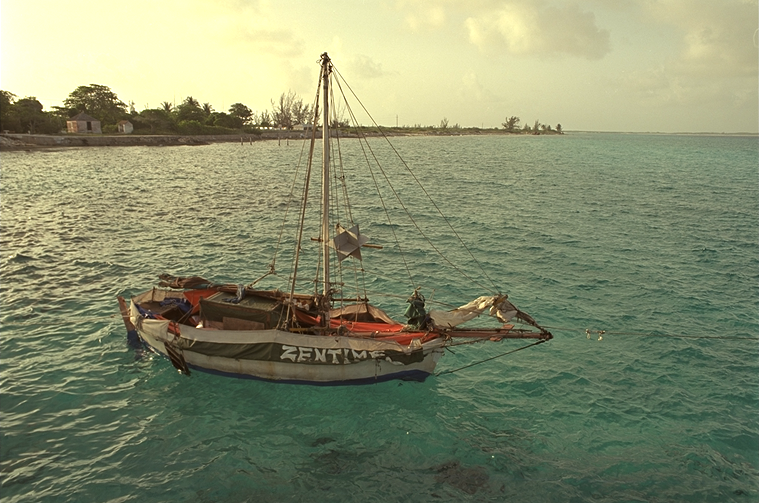
\includegraphics[width=0.9\textwidth]{figures/applying.png}
        \end{center}
    \end{frame}

    \begin{frame}[fragile]{Constraining Template Parameters}
        \framesubtitle{Applying Constraints}
        Both \emph{type} \& \emph{non-type template parameters} may be \emph{constrained} by using a \emph{requires clause}. The \emph{constraint expressions} on its right can be anything that evaluates to \texttt{bool} at compile-time. \emph{Instantiation} occurs \textbf{only} when the entire constraint expression evaluates \texttt{true}!
        \vspace{-1em}
        \begin{center}
        \begin{lstlisting}[caption={constraining types \& values by using the \texttt{requires} clause.}]
template<class T> requires Add<T>
T add(T x, T y) { return x + y; }

template<typename T> requires Number<T> class Matrix;



template<auto N> requires Even<N>
int square_even() { return N*N; } \end{lstlisting}
        \end{center}
    \end{frame}

    \begin{frame}[fragile]{Constraining Template Parameters}
        \framesubtitle{Applying Constraints}
        Both \emph{type} \& \emph{non-type template parameters} may be \emph{constrained} by using a \emph{requires clause}. The \emph{constraint expressions} on its right can be anything that evaluates to \texttt{bool} at compile-time. \emph{Instantiation} occurs \textbf{only} when the entire constraint expression evaluates \texttt{true}!
        \vspace{-1em}
        \begin{center}
        \begin{lstlisting}[caption={which even supports constraining C\texttt{++}20 generic lambdas!?}]
template<class T> requires Add<T>
T add(T x, T y) { return x + y; }

template<typename T> requires Number<T> class Matrix;
auto add = []<typename T>(T x, T y) requires Add<T> {
    return x + y;
};
template<auto N> requires Even<N>
int square_even() { return N*N; } \end{lstlisting}
        \end{center}
    \end{frame}

    \begin{frame}[fragile]{Concept Overload Resolution Rule}
        \framesubtitle{Applying Constraints}
        \begin{columns}
        \column{0.735\textwidth}
            Intuitively, the most \emph{constrained overload} will be chosen (i.e. with the \textbf{most} requirements). Since this is now part of ``official'' \emph{overload resolution}, and isn't a ad-hoc method like SFINAE; it gives an uniform syntax with the rest of the language. The amount of edge-cases, and hacks is reduced.
            \vspace{-1.5em}
        \column{0.265\textwidth}
            \begin{center}
                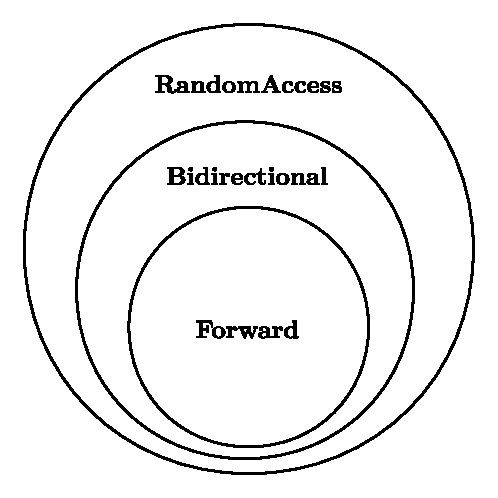
\includegraphics[width=\textwidth]{figures/iterators.eps}
            \end{center}
        \end{columns}
        \begin{center}
        \begin{lstlisting}[caption={function overloading for \texttt{advance} based on type constraint.}]
template<typename T> requires ForwardIterator<T>
void advance(T& iterator, std::size_t distance);

template<typename T> requires RandomAccessIterator<T>
void advance(T& iterator, std::size_t distance); \end{lstlisting}
        \end{center}
    \end{frame}

    \begin{frame}[fragile]{Logical Operations on Constraints}
        \framesubtitle{Applying Constraints}
        \begin{columns}
        \column{0.7\textwidth}
            The constraint expression can also be a logical summation of constraints by using \texttt{\&\&} and \texttt{||}. They are similar to logical operators, as should be no surprise. These evaluate to \texttt{true} when: \hfill
            \vspace{-0.9em}
            \begin{itemize}
                \item{\textbf{conjunctions:} \textbf{both} constraints satisfied,}
                \item{\textbf{disjunctions:}\ \textbf{at least one} was satisfied.}
            \end{itemize}
        \column{0.3\textwidth}
            \begin{center}
                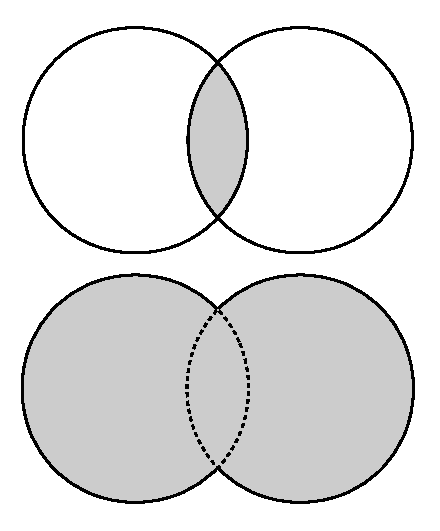
\includegraphics[width=0.815\textwidth]{figures/logical.eps}
            \vspace{1.0em}
            \end{center}
        \end{columns}
        \begin{center}
            \vspace{-1.0em}
            \begin{lstlisting}
template<typename T> requires is_integral_v<T> ||
                              is_floating_point_v<T>;
T add(T x, T y) requires Summable<T> { return x+y; }

template<auto N> requires Even<N> && Num<decltype(N)>
int square_even() { return N*N;  } // value & type N \end{lstlisting}
        \end{center}
    \end{frame}

    \begin{frame}[fragile]{Defining Constraints}
        \begin{center}
        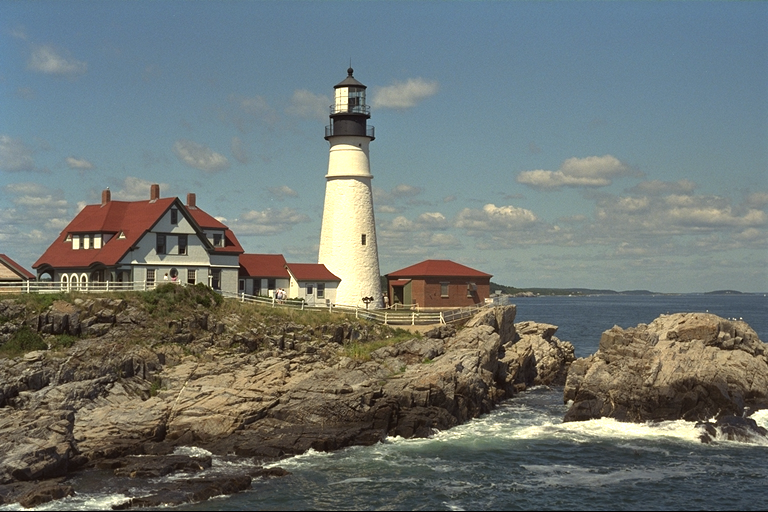
\includegraphics[width=0.9\textwidth]{figures/defining.png}
        \end{center}
    \end{frame}

    \begin{frame}[fragile]{Requirements}
        A list of syntactic \emph{requirements} for an template parameter can be checked by using an \emph{requires expression}. This expression evaluates to \texttt{true} when \textbf{all} requirements are \textbf{satisfied}. Artificial ``variables'' can be introduced, which have no linkage, storage or lifetime, and are only there for writing convenience (see e.g. \texttt{std::declval}).
        \framesubtitle{Defining Constraints}
        \begin{itemize}
        \item{\textbf{simple:} just asserts the validity of some expression \texttt{<expr>;},}
        \item{\textbf{type:} checks the validity of some type by a \texttt{typename} prefix,}
        \item{\textbf{compound:} validates the properties of some given expression,}
        \item{\textbf{nested:} specifies \textbf{more} requirements based on local variables.}
        \end{itemize}
    \end{frame}

    \begin{frame}[fragile]{Simple Requirements}
        \framesubtitle{Requirements}
        \begin{center}
        \begin{lstlisting}[caption={simple requirements in an incomplete \texttt{ForwardIterator}.}]
template<typename T>
concept ForwardIterator = requires {
    T{};
    T();
};
\end{lstlisting}
        \end{center}
    \end{frame}

    \begin{frame}[fragile]{Type Requirements}
        \framesubtitle{Requirements}
        \begin{center}
        \begin{lstlisting}[caption={type requirements in our incomplete \texttt{ForwardIterator}.}]
template<typename T>
concept ForwardIterator = requires {
    typename iterator_traits<T>::value_type;
    typename iterator_traits<T>::difference_type;
    typename iterator_traits<T>::reference;
    typename iterator_traits<T>::pointer;
    typename iterator_traits<T>::iterator_category;
}; \end{lstlisting}
        \end{center}
    \end{frame}

    \begin{frame}[fragile]{Compound Requirements}
        \framesubtitle{Requirements}
        \begin{center}
        \begin{lstlisting}[caption={compound requirements found in an \texttt{ForwardIterator}.}]
template<typename T>
concept ForwardIterator = requires(T x) {
    {  *x } -> iterator_traits<T>::reference;
    { ++x } -> T&;
    { x++ } -> T;
} && requires(T x, T y) {
    { std::swap(x, y) } noexcept;
}; \end{lstlisting}
        \end{center}
    \end{frame}

    \begin{frame}[fragile]{Nested Requirements}
        \framesubtitle{Requirements}
        \begin{center}
        \begin{lstlisting}[caption={usage of nested requirement in an \texttt{Allocatable} concept.}]
template<typename T>
concept Allocatable = requires(T x, std::size_t n) {
    requires Same<T*, decltype(&x)>;
    { x.<@\texttildelow @>T() } noexcept;
    requires Same<T*, decltype(new T)>;
    requires Same<T*, decltype(new T[n])>;
    { delete new T[n] };
    { delete new T };
}; \end{lstlisting}
        \end{center}
    \end{frame}

    \begin{frame}[fragile]{Naming Constraints}
        \framesubtitle{Defining Constraints}
        One can name \emph{complex constraints} into a \emph{concept} with \texttt{concept}. It's a glorified \texttt{constexpr bool} without Turing completeness :)
        \vspace{-0.7em}
        \begin{center}
        \begin{lstlisting}[caption={giving names to constraints by using the \texttt{concept} keyword.}]
template<typename T>
concept ForwardIterator = InputIterator<T> &&
                          DefaultConstructible<T> &&
                          EqualityComparable<T, T> &&
                          WeaklyIncrementable<T> &&
                          SwappableWith<T, T>;
template<typename T>
concept BidirectionalIterator = requires(T x) {
    { --x } -> T&;
    { x-- } -> T;
} && ForwardIterator<T>;
template<auto N> concept Even = (N % 2) == 0;\end{lstlisting}
        \end{center}
    \end{frame}

    \begin{frame}[fragile]{Defining ``Good'' Concepts}
        \framesubtitle{Defining Constraints}
        Some concepts are better than others. Many of the concepts here, are not ``good'' concepts. The core idea is that concepts should be defined to make types and algorithms 'plug compatible'. Which is:\hfill
        \vspace{0.8em}
        \begin{itemize}
            \item{to write \emph{algorithms} that can be used for a \emph{variety of types}, and}
            \item{to define \emph{types} that can be used with a \emph{variety of algorithms}.}
        \end{itemize}
        \begin{center}
        \emph{``the ideal is not minimal requirements, but requirements expressed in terms of fundamental and complete concepts.'' -- B.\ Stroustrup}
        \end{center}
    \end{frame}

    \begin{frame}[fragile]{Standard Library Concepts}
        Writing many of the ``boilerplate'' concepts isn't fun, and it's easy to get them wrong. Luckily, C\texttt{++}20 will be receiving a bunch from the \emph{Ranges TS}. Many of these we've defined in this presentation!!
        \vspace{1em}
        \begin{center}
        \begin{table}
        \begin{tabular}{cccc}
            \toprule
            \textbf{Core} & \textbf{Comparison} & \textbf{Object} & \textbf{Callable}\\
            \midrule
            Same & Boolean & Copyable & Invocable \\
            Integral & EqualityComparable & Movable & Predicate \\
            Swappable & StrictTotallyOrdered  & Regular & Relation \\
            Constructible & + $\cdots$With variants!   & Semiregular & WeakOrder \\
            \bottomrule
        \end{tabular}
        \caption{excerpt of the concept groups from the \texttt{<concepts>} header.}
        \end{table}
        \end{center}
    \end{frame}

    \begin{frame}[fragile]{Ranges TS Library}
        \framesubtitle{Standard Library Concepts}
        Many of the remaining concepts are found in the \emph{ranges library}, by \emph{Eric Niebler}, under the \texttt{<ranges>} header. e.g \texttt{InputIterator}. Along with them, we'll get a concepts-ready STL for C\texttt{++}20, which enable cool things like \emph{lazy evaluation} by using \emph{range views/actions}.
        \begin{center}
        \begin{lstlisting}[caption={example of the composability possibilities of range adaptors.}]
std::vector v { 10, 2, 6, 10, 4, 1, 9, 5, 8, 3 };
v = std::move(v) | action::sort | action::unique;
//  ---> v = { 1, 2, 3, 4, 5, 6, 8, 9, 10 } <--- 
auto range_of_v = v | view::remove_if([](int i) {
                          return i % 2 == 1; })
                    | view::transform([](int i) {
                          return to_string(i); })
                    | view::take(4);
// ---> range_of_v = { "2", "4", "6", "8" } <--- \end{lstlisting}
        \end{center}
    \end{frame}

    \begin{frame}[fragile]{Terse Syntaxes}
        \begin{itemize}
            \item{\textbf{Natural syntax} by \emph{Bjarne Stroustrup et al.}, which was part of the Concepts TS, and is implemented in \texttt{gcc}'s \texttt{-fconcepts}. Issues was related to ambiguous syntax and introducer syntax.}
            \item{\textbf{Concepts in-place syntax} by \emph{Herb Sutter}. In order to ``gain'' more consensus, removed ambiguity and dependent binding. It is forward-compatible with Bjarne syntax, but is a bit verbose.}
            \item{\textbf{Adjective syntax variants} by \emph{Thomas Köppe et al.}, after the Rapperswil \emph{``Bjarne / Herb stand-off''}, a new syntax: YAACD. It's essentially a constrained \texttt{auto}, and handles simpler cases.}
        \end{itemize}
    \end{frame}

    \begin{frame}[fragile]{Natural Syntax}
        \framesubtitle{Terse Syntaxes}
        \begin{center}
        \begin{lstlisting}
template<typename T> requires Sortable<T>
void sort(T& range);

template<Sortable T>
void sort(T& range);
void sort(Sortable& range);
void sort(RandomAccessIterator begin,
          RandomAccessIterator end);
auto sort = []<Sortable T>(T& r) { };
auto sort = [](Sortable& r) { };

BidirectionalIterator it = l.begin();

Mergeable{I1, I2, O}
O merge(I1 f1, I1 l1, I2 f2, I2 l2, O d); \end{lstlisting}
        \end{center}
    \end{frame}

    \begin{frame}[fragile]{Concepts In-Place Syntax}
        \framesubtitle{Terse Syntaxes}
        \begin{center}
        \begin{lstlisting}
template<typename T> requires Sortable<T>
void sort(T& range);

template<Sortable{T}>
void sort(T& range);
void sort(Sortable{}& range);
void sort(RandomAccessIterator{T} begin,
          T end);
auto sort = []<Sortable{T}>(T& r) { };
auto sort = [](Sortable{}& r) { };

BidirectionalIterator{T} it = l.begin();

template<Mergeable{I1, I2, O}>
O merge(I1 f1, I1 l1, I2 f2, I2 l2, O d); \end{lstlisting}
        \end{center}
    \end{frame}

    \begin{frame}[fragile]{Constrained \textbf{auto} Syntax}
        \framesubtitle{Terse Syntaxes}
        \begin{center}
        \begin{lstlisting}
template<typename T> requires Sortable<T>
void sort(T& range);

template<Sortable T>
void sort(T& range);
void sort(Sortable auto& range);
template<RandomAccessIterator T>
void sort(T begin, T end);
auto sort = []<Sortable T>(T& r) { };
auto sort = [](Sortable auto& r) { };

BidirectionalIterator auto it = l.begin();
template<class I1, class I2, typename O>
    requires Mergeable<I1, I2, O>
O merge(I1 f1, I1 l1, I2 f2, I2 l2, O d); \end{lstlisting}
        \end{center}
    \end{frame}

    \begin{frame}[fragile]{Concepts Summary}
        \framesubtitle{With post-Rapperswil Status!}
        \begin{itemize}
            \item{Generic programming for C\texttt{++} uses \emph{unconstrained templates}, which leads to \emph{horrible error messages}, and \emph{fragile interfaces}.}
            \item{Existing techniques (like SFINAE) are either \emph{insufficient},\ \emph{not easy to define},\ or have laughably \emph{obscure edge-cases} when it comes to defining, and using \emph{template parameter constraints}.}
            \item{With \emph{concepts} we can \emph{constrain template parameters} but not have to suffer from the problems above, by using its features:}
                \begin{itemize}
                    \item{\texttt{requires} \emph{clauses}, \texttt{requires} \emph{expressions} \& \emph{terse syntaxes}.}
                \end{itemize}
            \item{Generic programming in C\texttt{++}20 is a lot nicer using concepts!}
            \item{\textbf{Status:} Concepts, SLC/Ranges, Contracts, likely for C\texttt{++}20!}
        \end{itemize}
    \end{frame}

    \frame{\frametitle{Questions?} \begin{center}
        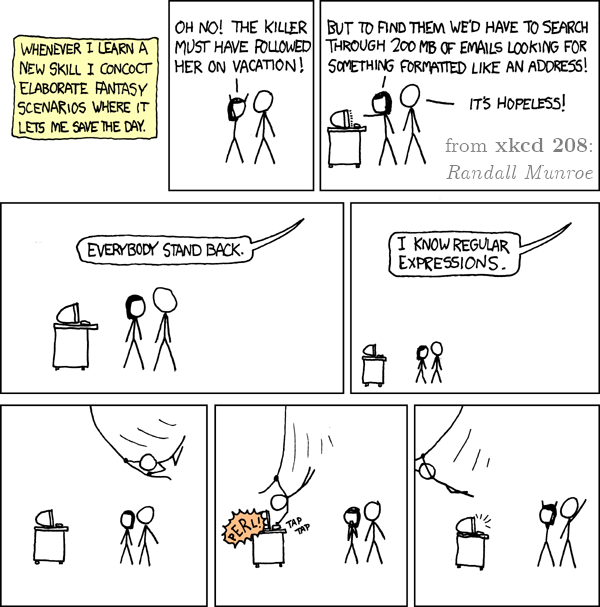
\includegraphics[height=0.85\textheight]
        {figures/regexs.png} \end{center} }
    \begin{frame}{References}
        \nocite{*}
        \bibliographystyle{alpha}
        \bibliography{slides}
    \end{frame}
    \frame{\frametitle{Acknowledgements}
        \begin{itemize}
            \item{\textbf{Concepts Lite in Practice} by \emph{R. Orr} (2016) for giving a nice and intuitive introduction to Concepts Lite TS at ACCU 2016. Some of the examples are taken from his slides and the article.}
            \item{\textbf{Generic Programming with Concepts} by \emph{A. Sutton} (2015), for presenting Concepts Lite from another angle. Many of the motivating example are based on those in his presentation too.}
            \item{I would like to thank \emph{P. Sommerlad}, for hosting the wonderful meeting in Rapperswil (2018), and allowing me to participate in the discussion on Concepts along with other topics in EWG.}
            \item{Finally, I would like to thank \emph{T. Lasser} and the other teachers and participants of ``Discovering and Teaching Modern C\texttt{++}''!}
        \end{itemize}
    }
\end{document}
